\documentclass[12pt, a4paper, oneside]{ctexart}
\usepackage{lmodern}
\usepackage{
	amsmath,
	amsthm,
	amssymb,
	bm,
	framed,
	graphicx,
	hyperref,
	mathrsfs,
	color,
	algorithm,
	xcolor,
	enumitem, % 添加此行以使用 enumitem 宏包
	fontspec, % 添加此行以使用 fontspec 宏包
	longtable,
	setspace,
}
\usepackage{subfigure}
\usepackage{graphicx}
\usepackage{subcaption}
\renewcommand{\tablename}{Table}
\usepackage{booktabs}
\linespread{1.5}

\definecolor{shadecolor}{RGB}{211,211,211}
\newcounter{problemname}

\newenvironment{problem}{
	\begin{shaded}
		\stepcounter{problemname}
		\par
		\noindent
		\textbf{\textsc{Problem} \arabic{problemname}. }
		\small
		}{
	\end{shaded}\par
}

% --------------------------------------------------------------------------------
\usepackage{sourcecodepro}
\usepackage{listings}
\usepackage{fontspec}
% \setmonofont{JetBrains Mono}
% \setmonofont{Courier New}
\lstdefinestyle{mystyle}{
	backgroundcolor=
	\color[RGB]{211,211,211}
	, % 更浅的背景色
	basicstyle=\ttfamily\small, % 代码字体和大小
	columns=flexible, % 柔性列宽
	breaklines=true, % 自动换行
	numbers=left, % 显示行号
	numberstyle=\tiny
	\color[RGB]{152,152,152}
	, % 行号颜色:浅灰色
	lineskip=2pt, % 调整行间距
	xleftmargin=1.5em, % 左边距
	framexleftmargin=1.5em, % 行号与代码框之间距离
	rulecolor=
	\color[RGB]{224,224,224}
	, % 框线颜色:浅灰色
	keywordstyle=
	\color[RGB]{33,150,243}
	\bfseries, % 关键字颜色:Material蓝色并加粗
	commentstyle=
	\color[RGB]{76,175,80}
	\itshape, % 注释颜色:Material绿色并斜体
	stringstyle=
	\color[RGB]{255,87,34}
	, % 字符串颜色:Material深橙色
	numbersep=10pt, % 行号与代码间距
	identifierstyle=
	\color[RGB]{33,33,33}
	, % 普通标识符颜色:深灰色
	emphstyle=
	\color[RGB]{156,39,176}
	, % 突出显示颜色:Material紫色
	emph={self, init, class, def}, % 自定义突出显示的标识符
	ndkeywordstyle=
	\color[RGB]{255,193,7}
	, % 内置函数颜色:Material黄色
	ndkeywords={print, range, len, int, str, float, bool}, % 内置函数列表
	morekeywords={True, False, None}, % 更多关键字
	tabsize=4, % Tab 宽度
	showspaces=false, % 不显示空格
	frame=single, % 外框样式
	showstringspaces=false, % 不显示字符串中的空格
	captionpos=b, % 标题位置:底部
}


\begin{document}
\title{BME2104 HW\#1\textbf{
		Imaging Foundation}}

\author{Zhihao Zhang, 2024291074\\ \textit{zhangzhh12024@shanghaitech.edu.cn}}
\date{Mar. 27, 2025}
\maketitle

\begin{problem}

A cycle of a square wave can be expressed as following equation

\[f(x)=\left\{\begin{array}{cc}1,&0\leq x<1/2\\0,&1/2\leq x<1\end{array}\right.\]

Using Fourier Series, please do analytical derivation to prove that this square wave can be represented as a linear combination of sine waves of different frequencies.

Then, using a programming environment of your choice (MATLAB/Python), please build a numerical model to demonstrate that the above square wave is indeed a linear combination of sine waves. Please use plots to help explain.

\end{problem}
\subsection*{Solution 1}
% Add your solution here

For a periodic function with period 1, the Fourier series is given by:
\[f(x) = \frac{a_0}{2} + \sum_{n=1}^{\infty} [a_n \cos(2\pi n x) + b_n \sin(2\pi n x)]\]

Where the coefficients are:
\begin{align}
	a_0 & = 2\int_0^1 f(x)dx              \\
	a_n & = 2\int_0^1 f(x)\cos(2\pi nx)dx \\
	b_n & = 2\int_0^1 f(x)\sin(2\pi nx)dx
\end{align}

For the given square wave:
\begin{align}
	a_0 & = 2\int_0^1 f(x)dx = 2\int_0^{1/2} 1\,dx + 2\int_{1/2}^1 0\,dx = 1                                       \\
	a_n & = 2\int_0^{1/2} \cos(2\pi n x)dx = \frac{\sin(\pi n)}{\pi n} = 0                                         \\
	b_n & = 2\int_0^{1/2} \sin(2\pi n x)dx = \frac{1 - \cos(\pi n)}{\pi n} = \begin{cases}
		                                                                         \frac{2}{\pi n}, & \text{for odd } n  \\
		                                                                         0,               & \text{for even } n
	                                                                         \end{cases}
\end{align}

Therefore, the Fourier series representation is:
\[f(x) = \frac{1}{2} + \frac{2}{\pi}\sum_{k=0}^{\infty} \frac{1}{2k+1}\sin(2\pi(2k+1)x)\]



Python implementation to visualize the Fourier approximation:

\begin{lstlisting}[style=mystyle,language=Python]
	def fourier_square(x, harmonics):
    # Start with the constant term a0 = 1/2
    f_approx = 0.5 * np.ones_like(x)
    for k in range(harmonics):
        n = 2 * k + 1  #  odd only
        f_approx += (2 / (np.pi * n)) * np.sin(2 * np.pi * n * x)
    return f_approx
\end{lstlisting}


\begin{figure}[htbp]
	\centering
	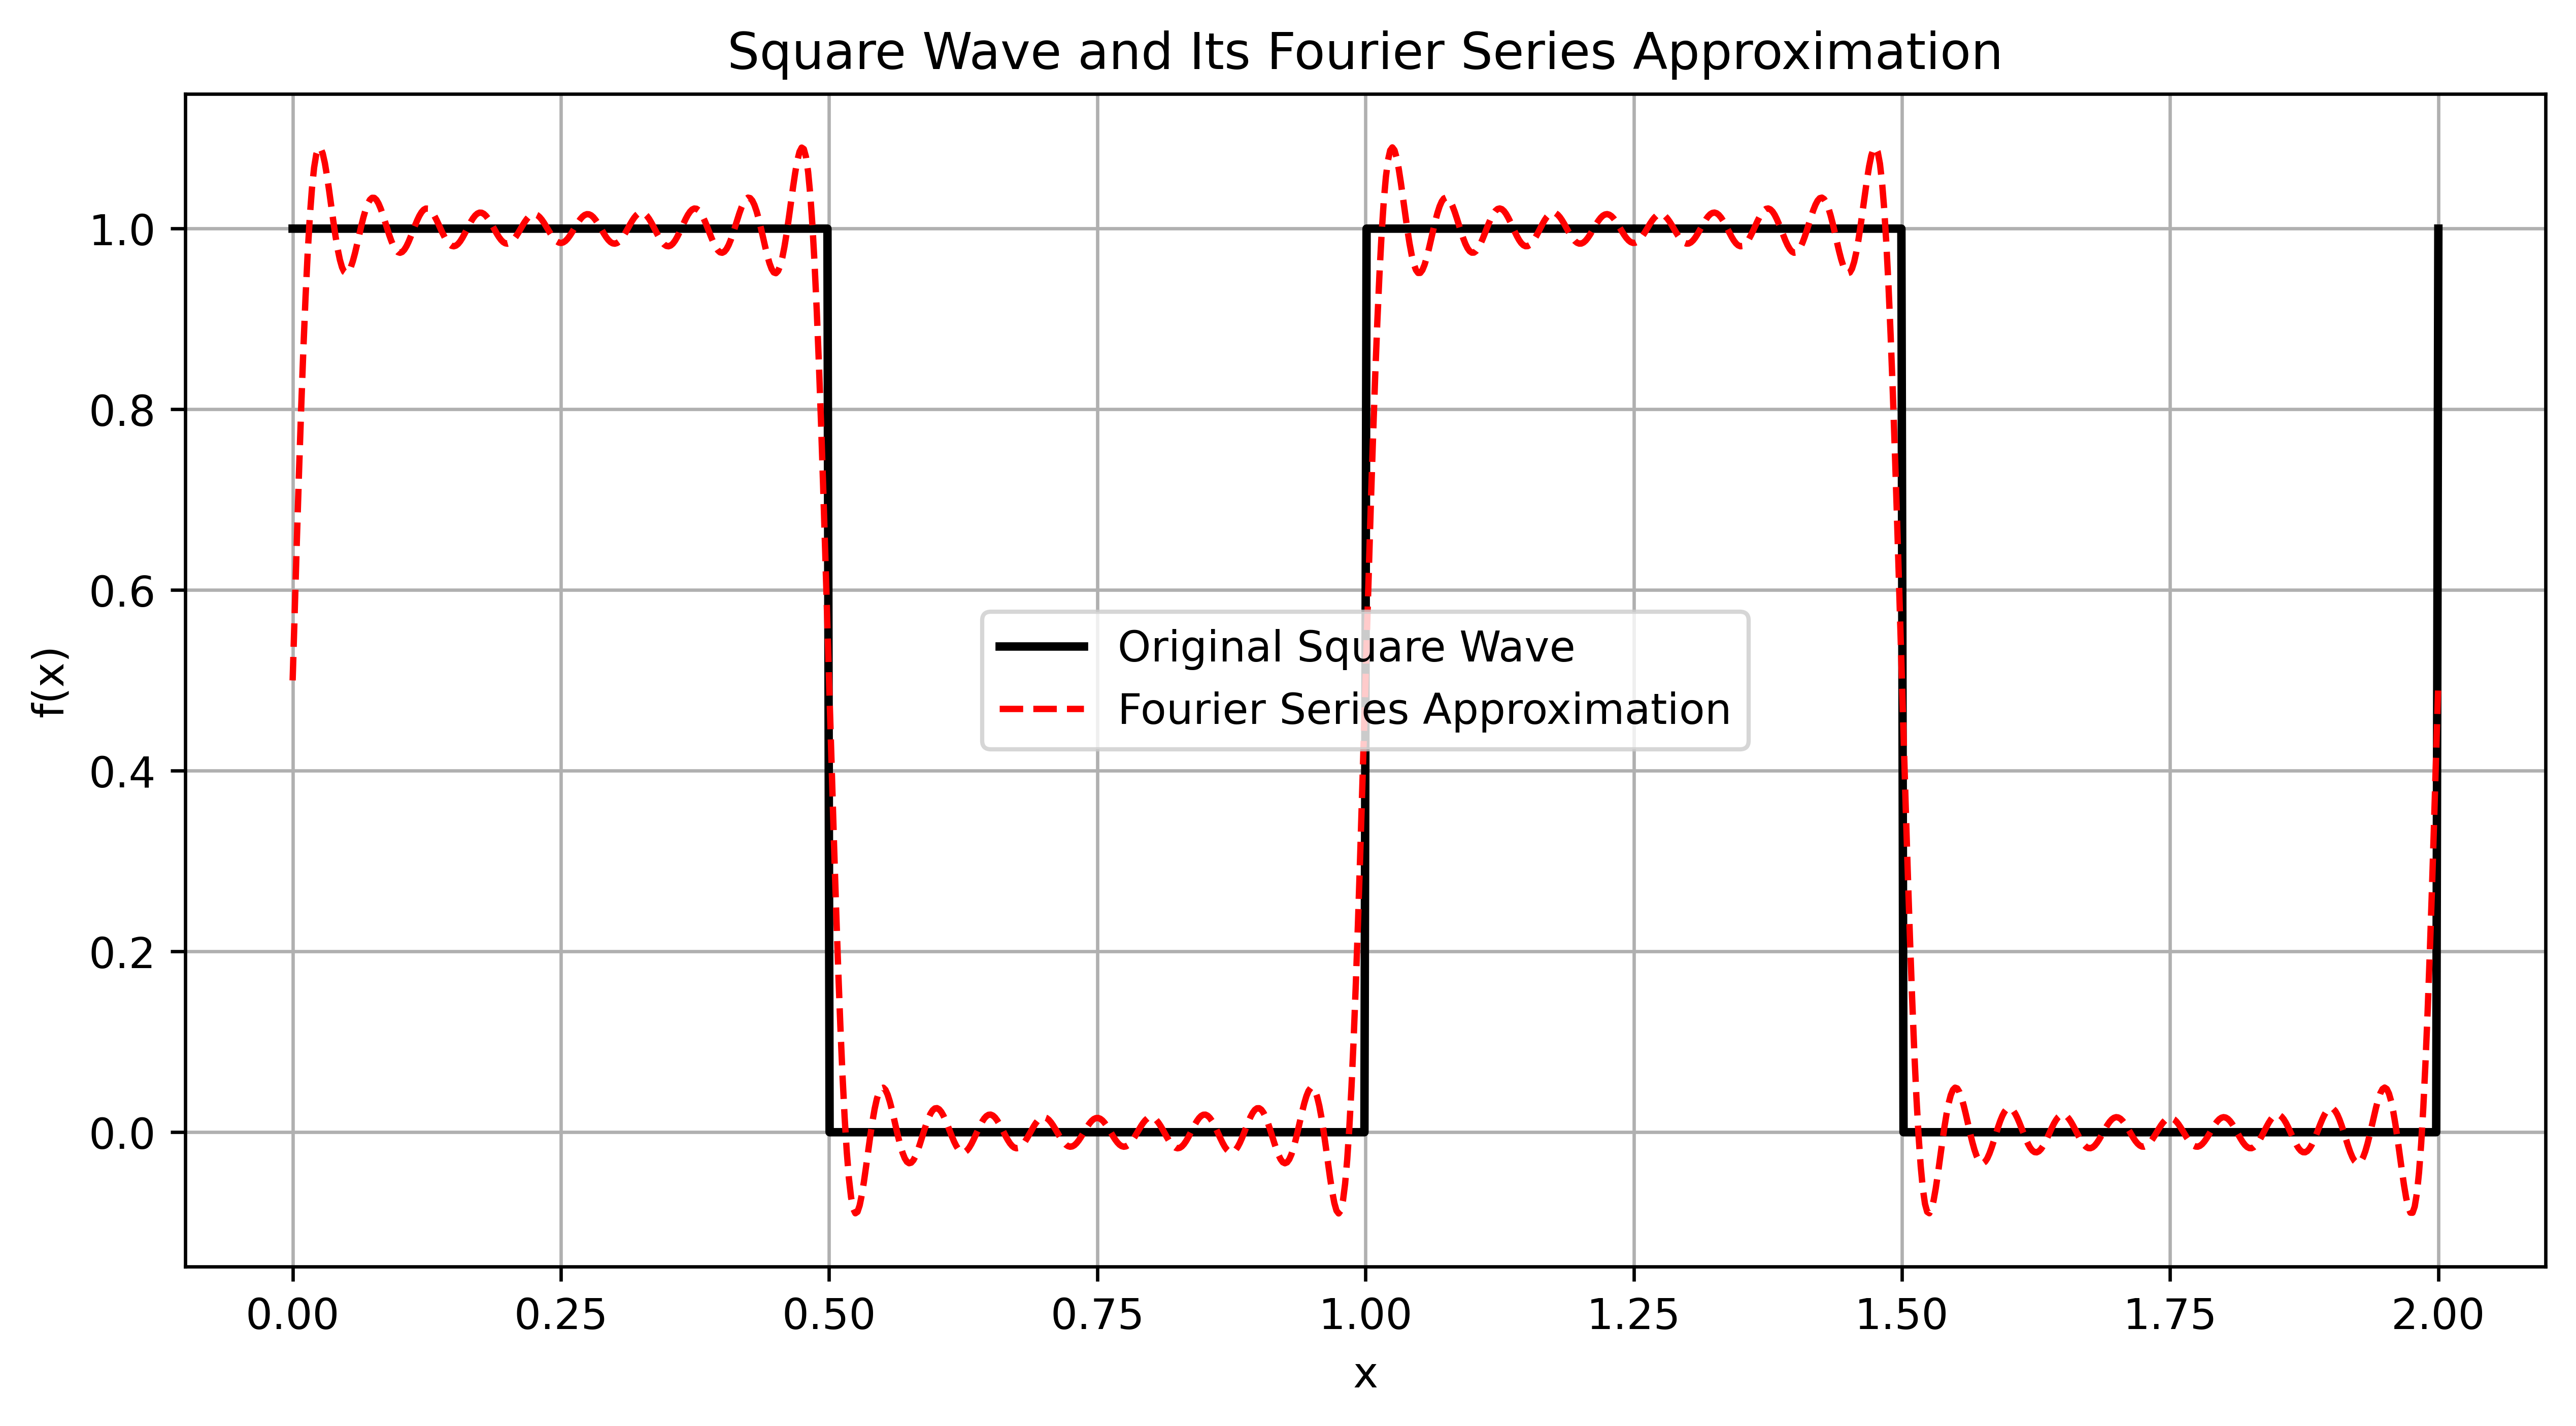
\includegraphics[width=1\textwidth]{result/square_wave_fourier.png}
	% \caption{fourier}
	% \label{fig:fourier}
\end{figure}


% \begin{figure}[h]
% 	\centering
% 	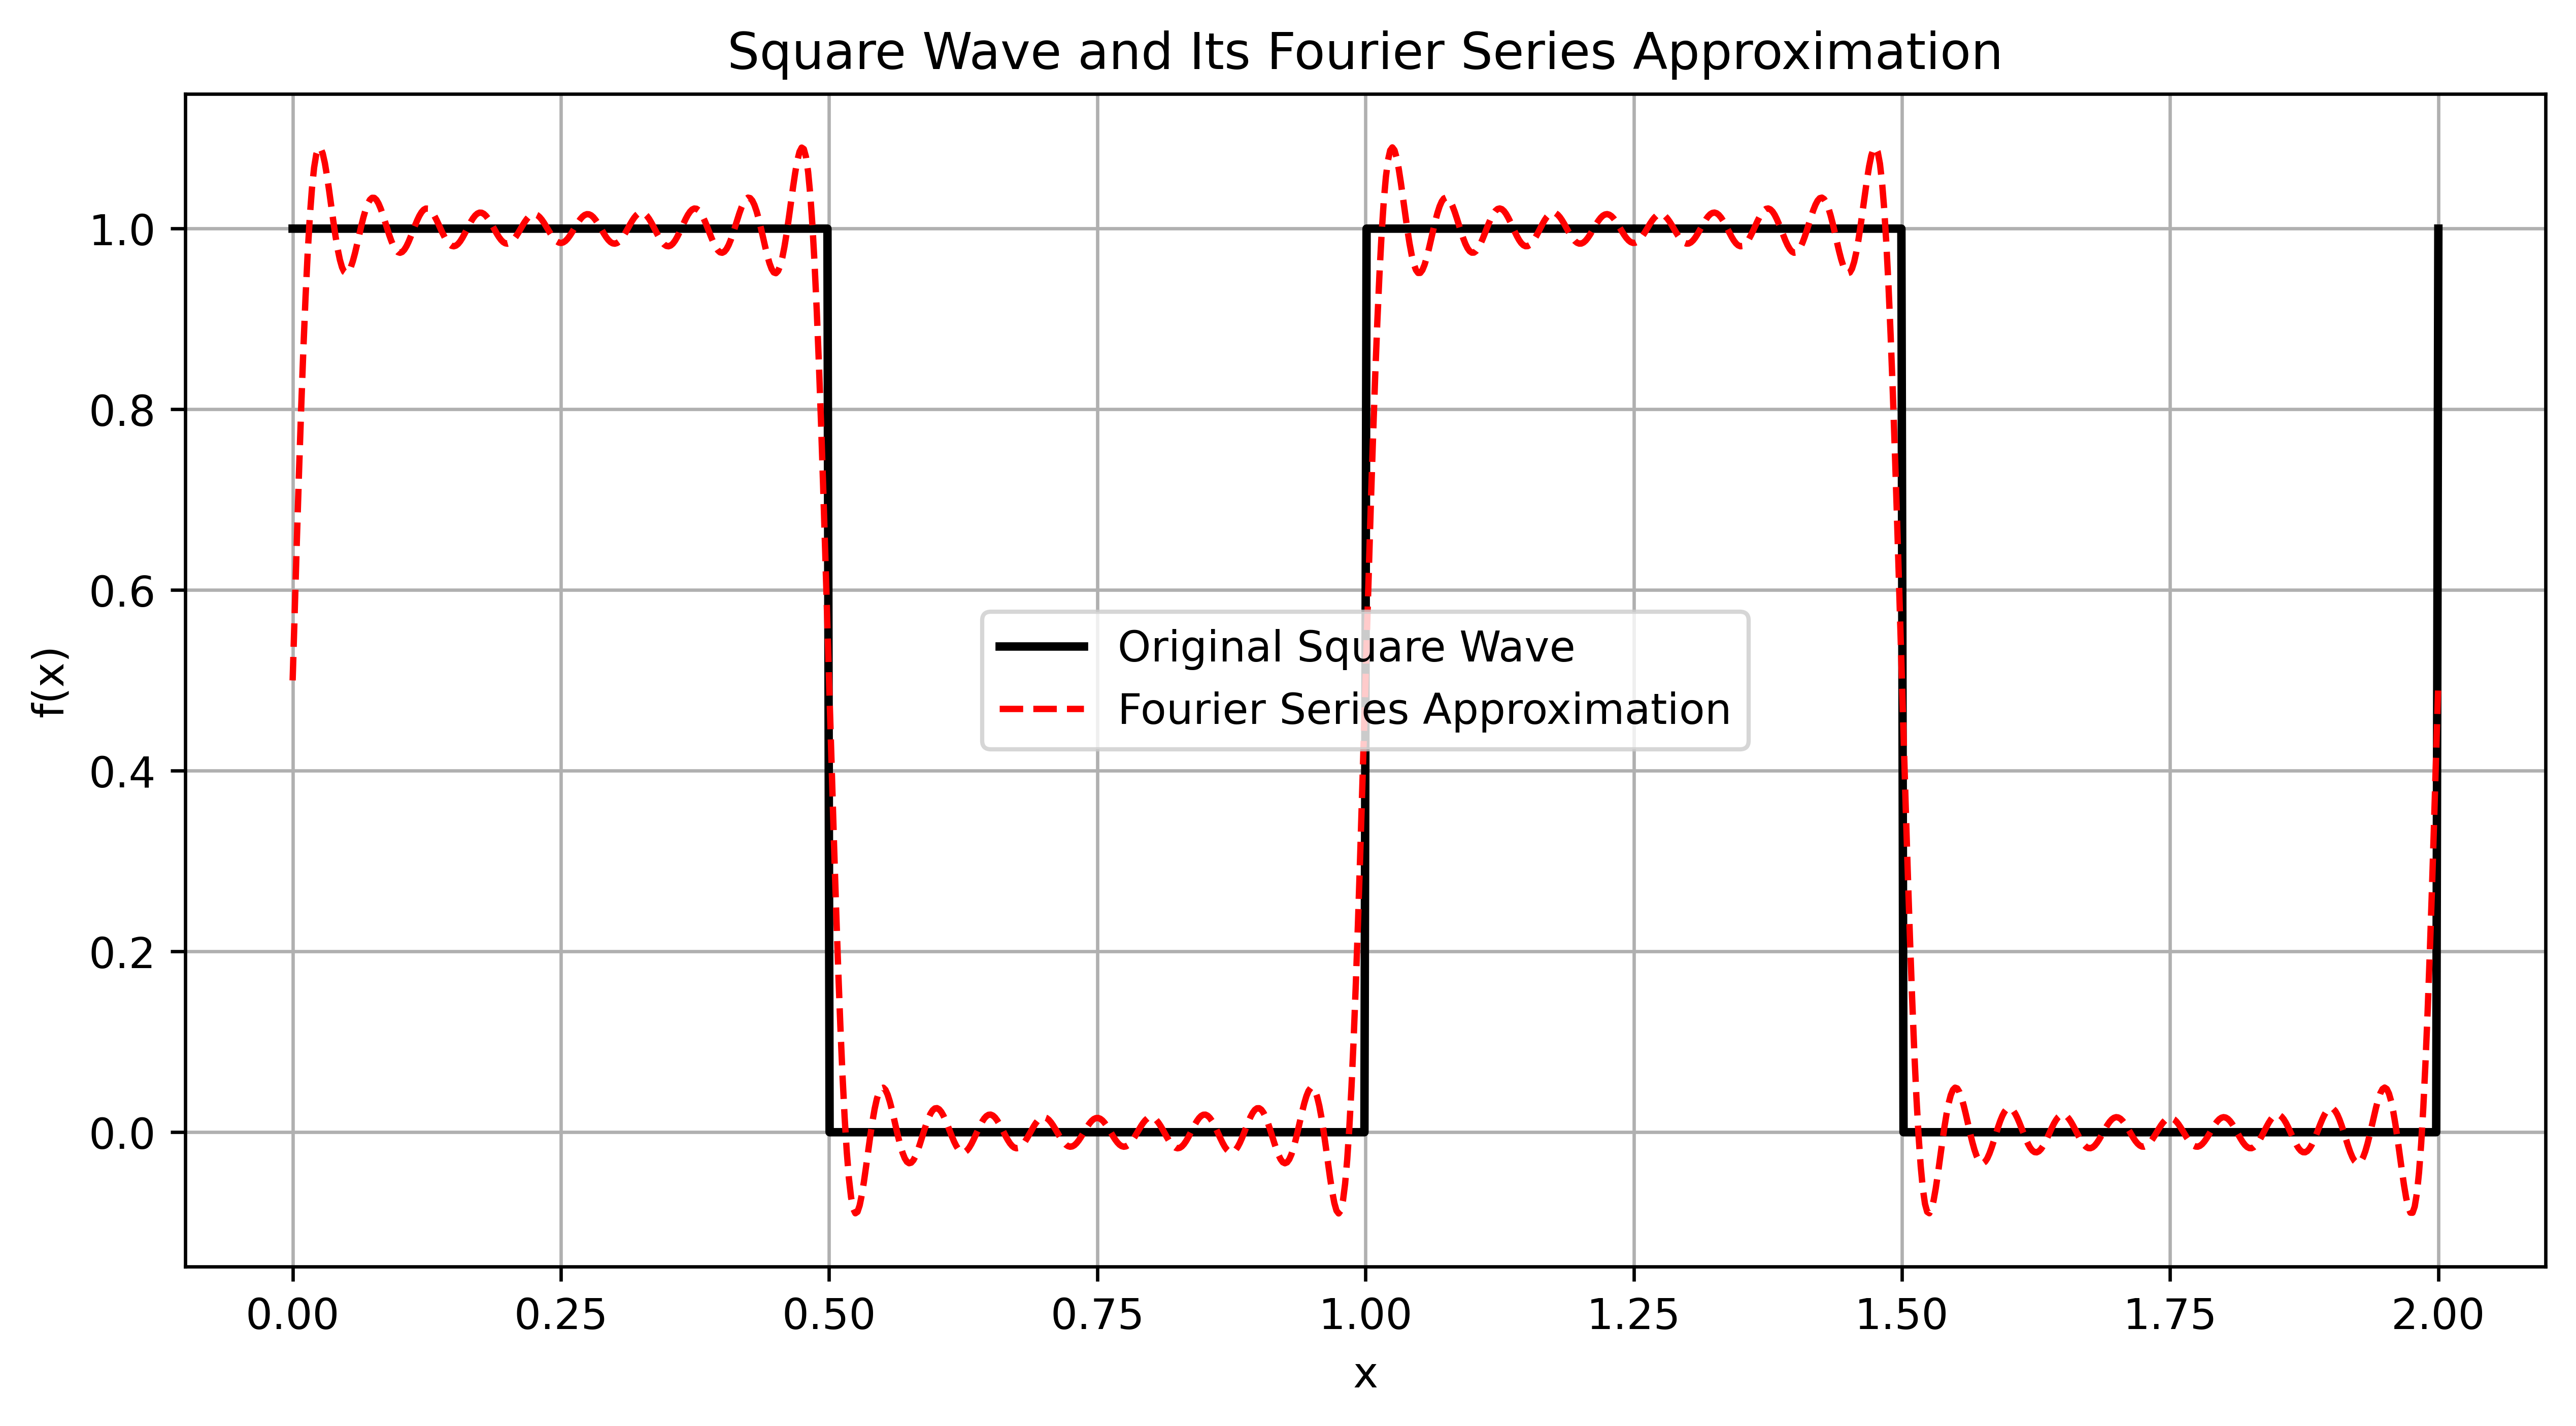
\includegraphics[width=0.8\textwidth]{./result/square_wave_fourier.png}
% 	\caption{Fourier series approximation of square wave. As more terms are added, the approximation becomes closer to the original square wave, demonstrating that the square wave is indeed a linear combination of sine waves.}
% \end{figure}



From both the analytical derivation and numerical demonstration, we've shown that the square wave can be represented as a linear combination of sine waves of different frequencies. We observe that:
\begin{itemize}[itemsep=-3pt, parsep=0pt]
	\item Only odd-numbered harmonics contribute to the series
	\item The amplitude of each harmonic decreases as $1/n$
	\item More terms lead to better approximation, especially at discontinuities
	\item The Gibbs phenomenon causes oscillations near the discontinuities
\end{itemize}



\begin{problem}

A micro-CT imaging system’s spatial resolution was characterized with a thin tungsten wire phantom. An axial micro-CT slice image of the phantom is shown here (original image file is uploaded to Blackboard, ” MTF-slice”. Note the pixel size is 7.6um).

(1). Please plot the Line Intensity Profile (LIP) of the wire in the center of the image. Please fit the LIP with a Gaussian function.
(2). Assume that the diameter of the wire is very small, therefore the LIP can be assumed to be the LSF of the micro-CT. Using the LSF, please calculate the MTF of the micro-CT.  Please plot the MTF, and fit your MTF with a Gaussian function.  Is your Gaussian function in (2) close to the FT (Fourier Transform) of the Gaussian function in (1)? Find your spatial resolution at 10\% MTF? Explain your result.


\end{problem}
\subsection*{Solution 2}
% Add your solution here


Line Intensity Profile (LIP) is defined as the intensity of the image along a line, which can be represented as a function of distance from the center of the wire.


% \[f(x) = a \cdot e^{-\frac{(x-b)^2}{2c^2}} + d\]



The key Python code and the result is as follows:

\begin{lstlisting}[style=mystyle,language=Python]
	# Get the center row of the image
	center_row = img[img.shape[0] // 2, :]

	# Define Gaussian function for fitting
	def gaussian(x, amplitude, mean, sigma):
		return amplitude * np.exp(-((x - mean) ** 2) / (2 * sigma**2))

	# Fit Gaussian to LIP
	popt, _ = curve_fit(gaussian, x, center_row)
	fitted_gaussian = gaussian(x, *popt)

\end{lstlisting}


\begin{figure}[h]
	\centering
	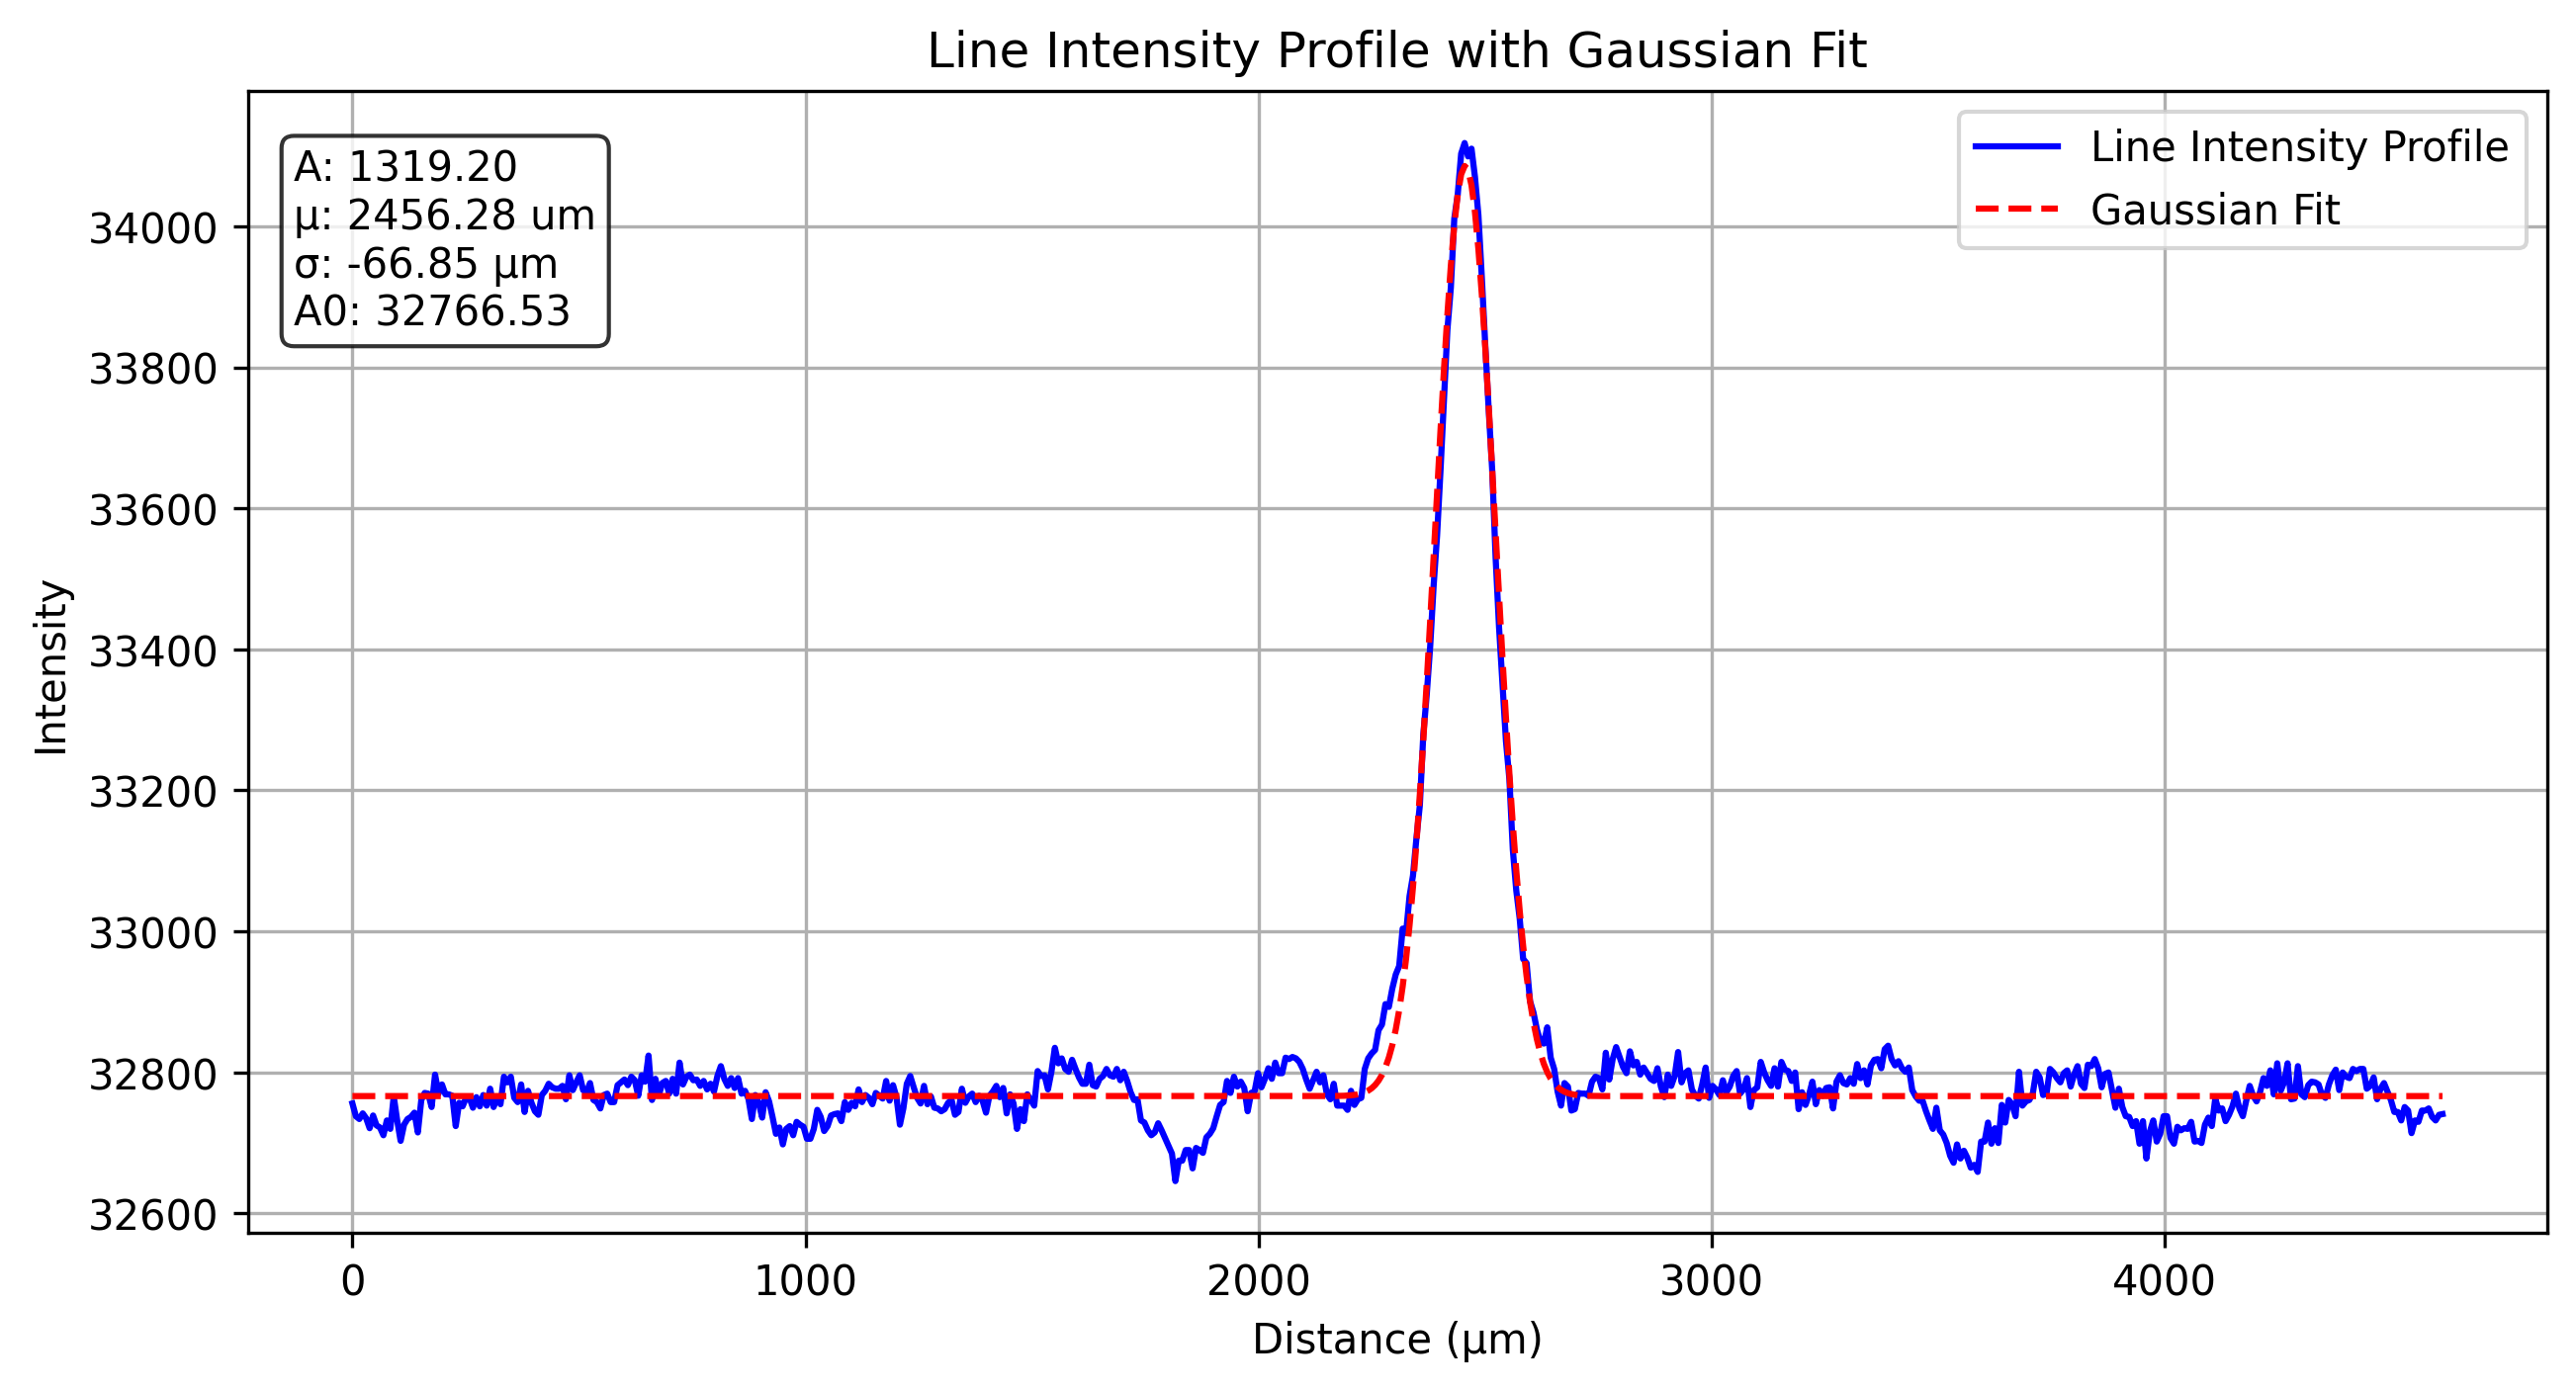
\includegraphics[width=1\textwidth]{./result/lip_gaussian_fit.png}

\end{figure}

% The Gaussian fit parameters were:
% \begin{align}
% 	a & = \text{X}    \\
% 	b & = \text{X}    \\
% 	c & = \text{X μm} \\
% 	d & = \text{X}
% \end{align}


Line Spread Function (LSF) is the response of the imaging system to a point source. The LSF can be derived from the Line Intensity Profile (LIP) by taking the derivative of the Gaussian function fitted to the LIP.


\[LSF(y) = \frac{1}{\sqrt{2\pi\sigma^2}} \exp\left(-\frac{(y - y_0)^2}{2\sigma^2}\right)\]



% The Full Width at Half Maximum (FWHM) of the fitted Gaussian is $2.355 \cdot c = \text{X μm}$.



\begin{problem}

Start with any noisy digital image (it can be downloaded from the web, synthesized by yourself, or even an image in your smartphone), first convert it into 8-bit grey scale if it is not already so, then re-size it to 512 x 512 using digital down-sampling or up-sampling (combined with cropping/padding if necessary), you will end up with a noisy grey-scale image of 512 x 512. Then, do image denoising using the following two approaches:

(1). Filtering in frequency space: First find the FT version of the image, then multiply the FT version with a low-pass filter, which will give you a filtered FT version. Finally do an inverse FT to yield the denoised image.  Please try with low-pass filters of different filtration levels, and show your results.

(2). Filtering in image space: design a ‘smoothing/denoising’ filter kernel, and convolute it with the noisy grey-scale image to receive your denoised image.

(3). For the above two denoising approaches, calculate their respective MSE, PSNR, and SSIM relative to the original image before denoising.

\end{problem}


\subsection*{Solution 3}
% Add your solution here



\end{document}

\end{document}